% !TEX root = omar-thesis-proposal.tex
\vspace{-25pt}
\section{Motivation}\label{motivation}
%\begin{quote}\textit{The recent development of programming languages suggests that the simultaneous achievement of simplicity 
%and generality in language design is a serious unsolved 
%problem. }
%- Reynolds, 1970\todo{citations}\end{quote}
%%One might exp ``generality''
Specifying and implementing a ``general purpose'' programming language and its associated tools (collectively, a \emph{programming system}) has long been a grand challenge in computing. Were a truly general system to emerge, we might expect that its users would rarely  need to develop a new dialect of the system. Embeddings of new abstractions using mechanisms built into the language would be suitably reasonable, natural and performant. Alas, new language and tool dialects spanning all major language lineages continue to be widely used as vehicles for new abstractions (examples of which we will discuss throughout this work), suggesting that not all useful  abstractions can be seen, when considered comprehensively, as mere modes of use of any contemporary ``general purpose'' programming system.% The problem of achieving both simplicity and generality simultaneously with a single system remains unsolved. 

We observe that new dialects are often motivated by the desire to introduce new syntax, strengthen the language's static semantics or provide specialized editor services, all aspects of existing systems that appear fixed when considered from within (that is, from the perspective of a library provider). %, encouraged  historically  by the availability of tools like compiler generators and,  more recently, language workbenches \cite{workbenches} and DSL frameworks \cite{dsl}. Unfortunately, taking this approach makes it substantially more difficult for clients to import high-level abstractions orthogonally. 
It follows then that {language-integrated mechanisms} that allow library providers to extend these features of the system could strengthen its claim to generality by decreasing the need for new language and tool dialects. However, such mechanisms must be introduced with care, because decentralizing control over such fundamental aspects of the system could weaken its metatheory and permit ambiguities and conflicts when two libraries are combined (collectively, \emph{safety issues}). It could also make it more difficult to define new functions over expression forms in the language (the \emph{expression problem}) and make it more difficult to  understand the meaning of programs. 
In this thesis, we aim to show that by associating system extensions with types (forming what we call \emph{active types}) rather than new expression forms, and using a \emph{bidirectional type system} that enforces critical  abstraction barriers between extensions, we can  give abstraction providers the ability to orthogonally implement new syntax, type systems and editor services from within libraries, rather than as new language and tool dialects, while avoiding safety issues and retaining  an essentially conventional typing discipline. %We call user-defined types that introduce new features into the system in this way \emph{active types}.  % also highly expressive.
%But taking a \emph{language-internal approach} to implementing a feature is the most practical. If a feature can be realized by creatively using existing language constructs and distributed as a library, clients face fewer barriers to adoption because it is easy to integrate library-based features into existing projects gradually and granularly and they leverage well-understood and well-developed mechanisms.
% But taking this approach is often \emph{not} possible today %We call designs \emph{monolithic programming systems}.

%To realize a new abstraction or system behavior, such experts can consider either a \emph{language-internal approach}, where they work within an existing language and distribute their solutions as libraries, or a \emph{language-external approach}, where they create a new, distinct programming system (often centered around what has come to be called a new \emph{domain-specific language} \cite{dsl}) or extend an existing system by some mechanism that is not part of the language itself, such as an extension mechanism supported by a {particular} compiler, editor or other tool.
\subsection{Motivating Example: Regular Expressions}\label{regex}
To make the problems we aim to address more concrete, we begin with a simple example that we will return to throughout this work. \emph{Regular expressions} are commonly used to express patterns in strings (e.g. DNA sequences) \cite{Thompson:1968:PTR:363347.363387}. Programmers who work with regular expressions regularly might want a programming system supporting features like:

\begin{enumerate}
\item \textbf{Syntax for pattern literals}. An ideal syntax would permit us to express patterns in a concise, conventional manner. For example, The BisI restriction enzyme cuts DNA whenever it sees the pattern \texttt{GC\textit{N}GC}, where \texttt{\textit{N}} represents any base. We would want to express it, perhaps, as follows (using curly braces to splice one pattern into another):
\begin{lstlisting}[numbers=none]
let N : Pattern = <SURLA|T|G|CEURL>
let BisI : Pattern = <SURLGC{EURLNSURL}GCEURL>\end{lstlisting}
%The cognitive load of reading and writing patterns is low and patterns are parsed once at compile-time. 
We would want malformed patterns to result in intelligible {compile-time} errors.
\item A \textbf{type system} that ensures that key invariants related to regular expressions are statically maintained:
	\begin{enumerate}
	\item only other patterns and properly escaped strings are spliced into a pattern, to avoid splicing errors and injection attacks \cite{owasp2013, Bravenboer:2007:PIA:1289971.1289975}
	\item out-of-bounds backreferences to a captured group are not used \cite{spishak2012type}
	\item string processing operations do not lead to a string that is malformed, when well-formedness can be captured as membership in a regular language \cite{fulton-thesis,HosoyaVouillonPierce2000ICFP}
	\end{enumerate}
%When an error is found, an intelligible error message is provided.
%\item An \textbf{implementation} that partially or fully compiles known regular expressions into the efficient internal representation that will be used by the regular expression matching engine (e.g., a finite automata \cite{Thompson:1968:PTR:363347.363387}) ahead of time. In most languages, this compilation step occurs at run-time, even if the pattern is fully known at compile-time, thereby introducing performance overhead into programs. If the developer is not careful to cache compiled representations, regular expressions used repeatedly in a program might be needlessly re-compiled on each use. %By performing this step ahead-of-time, these dangers can be avoided.
\item \textbf{Editor services} to support syntax highlighting, documentation, interactive testing and pattern extraction from example strings.
\end{enumerate}

%In a conventional \emph{monolithic} programming system, support for each of these features would need to be built into the language and tools. 
No system today builds in support for all of the features enumerated above in their strongest form, so library providers must provide support for regular expressions by leveraging  general-purpose mechanisms. Unfortunately, it is impossible to completely define the syntax and the specialized static semantics referenced above in terms of general-purpose notations and abstractions, so library providers need to compromise. 

The most common strategy is to ask clients to enter patterns as strings, deferring their parsing, typechecking, compilation and use all to run-time. This provides only a partial approximation to feature 1 (due to clashes between string escape sequences and regular expression syntax). None of the static guarantees can be provided in this way, leading to run-time exceptions (even in well-tested code \cite{spishak2012type}), and logic errors that cannot even be caught at run-time, some of which can lead to security vulnerabilities (due to injection attacks \cite{owasp2013}). It also introduces performance overhead due to run-time parsing and compilation of patterns, and redundant run-time checks. 

Requiring that clients instead introduce patterns directly using general-purpose constructs like sums or products (as exposed by, e.g., functional datatypes or objects) or operations over an abstract type, rather than via strings, provides only feature 2a at the expense of the weak approximation to feature 1 that the use of string literals provided. 

None of these approaches address the issue of tool support (feature 3). Regular expressions are not trivial to work with, and we have found that tool support can be quite helpful, even for professional programmers \cite{Omar:2012:ACC:2337223.2337324}. Indeed, a number of tools are available online that provide services like syntax highlighting, testing and explanations of patterns \cite{regexr} and pattern extraction from examples (e.g. \cite{_txt2re:_????}). Unfortunately, tools that must be accessed externally are difficult to discover and are thus used infrequently \cite{Murphy-Hill:2011:PIE:1958824.1958888,Campbell:2008:DRT:1636642.1636651,Omar:2012:ACC:2337223.2337324}. We found that they are also less usable than editor-integrated tools %(e.g. \cite{IntelliJRegexp}) 
because they require the programmer to switch contexts  and cannot make use of the code context \cite{Omar:2012:ACC:2337223.2337324}. Working with high-level abstractions in a ``low-level'' editor is thus awkward and error-prone, just like attempting to work with high-level abstractions in a low-level language. For these reasons,   we consider editor behavior as within the scope of an abstraction's specification.
\subsection{Language-External Approaches}\label{external-approaches}
\begin{figure}
\begin{center}
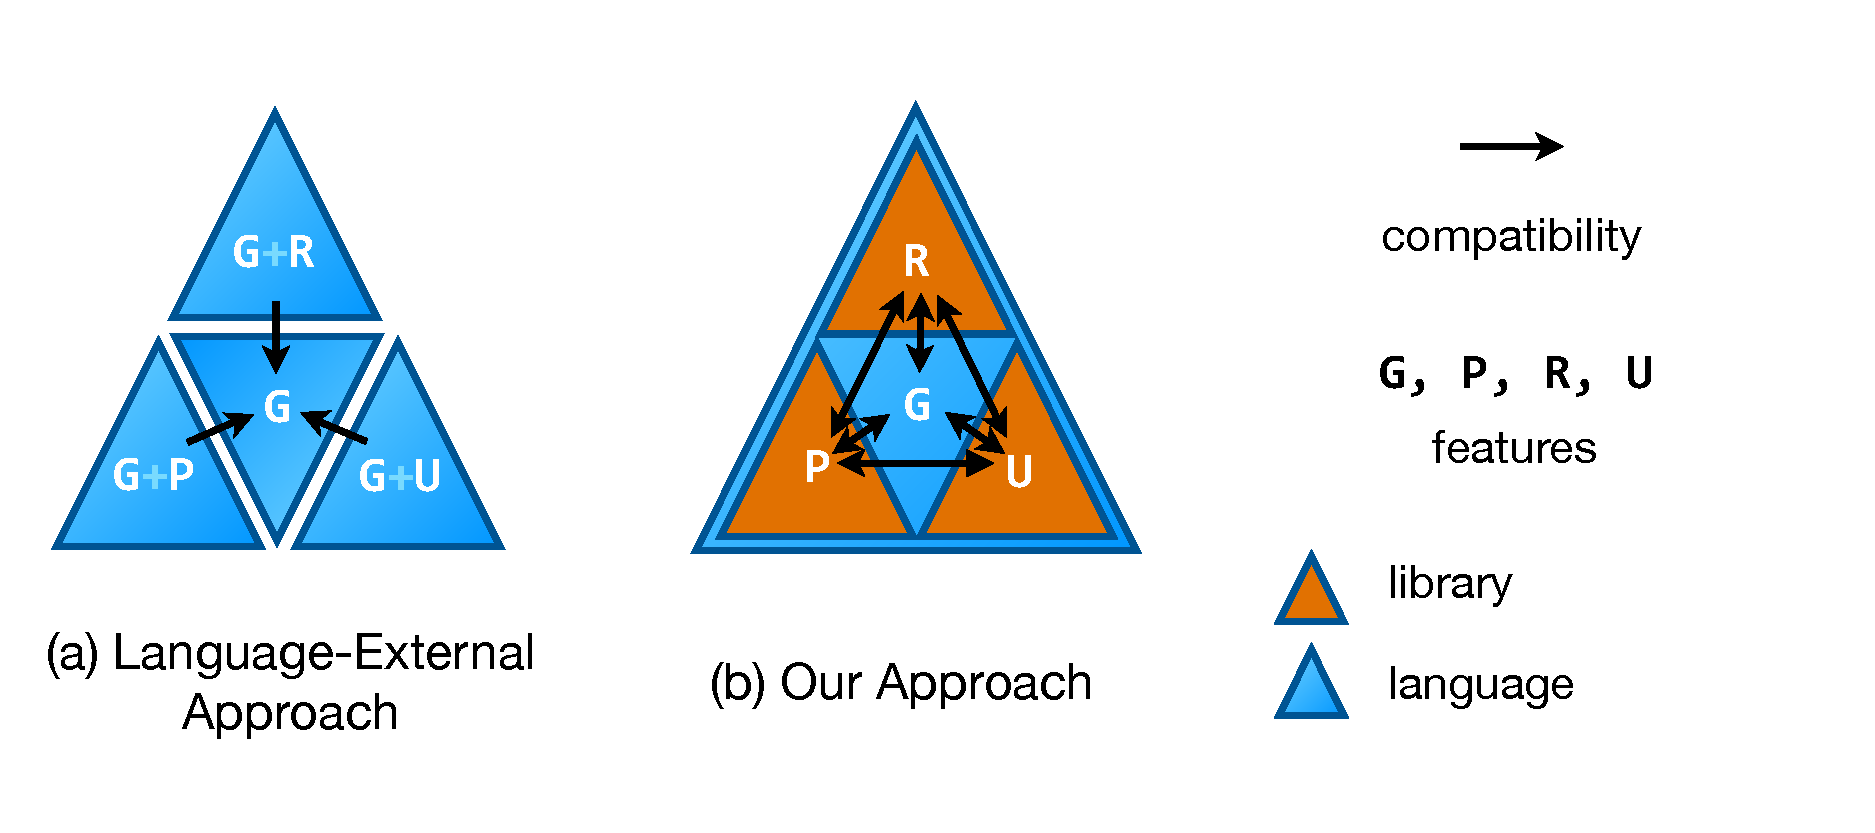
\includegraphics[scale=.48]{approaches.pdf}
\end{center}
\vspace{-20px}
\caption{\small (a) When taking a language-external approach, new features are packaged together into separate languages and tools, causing problems with orthogonality and client compatibility (described in the text). (b) When taking a language-integrated approach, there is one extensible host language and the compile-time and edit-time logic governing new constructs is expressed within ``active libraries''. If the extension mechanism precludes conflicts by construction, the problems of orthogonality and client compatibility are avoided.}
\label{approaches}
%\vspace{-10px}
\end{figure}

When the syntax and semantics of a system must be extended to fully realize a new feature providers typically take a \emph{language-external approach}, either by developing a new system dialect (supported by \emph{compiler generators} \cite{brooker1963compiler}, \emph{language workbenches} \cite{erdweg2013state}, \emph{DSL frameworks} \cite{fowler2010domain}, or simply be forking an existing codebase), or by using an extension mechanism for a {particular} compiler\footnote{Compilers that modify, or allow modification of, the semantics of their base language, rather than simply permitting semantics-preserving optimizations, should be considered a pernicious means for creating new languages. That is, some programs that purport to be written in C, Haskell or Standard ML are actually written in compiler-specific dialects of these languages.}, editor or other tool. For example, a researcher interested in providing regular expression related features (let us refer to these collectively as \texttt{R}) might design a new system with built-in support for these, perhaps basing it on an existing system containing some general-purpose features (\texttt{G}). A different researcher developing a new language-integrated parallel programming abstraction (\texttt{P}) might  take the same approach. A third researcher, developing a type system for reasoning about units of measure (\texttt{Q}) might again do the same. This results in a collection of distinct systems, as diagrammed in Figure \ref{approaches}a. This might be entirely sufficient if developing a proof of concept is the only goal, but it makes it difficult to achieve adoption of these abstractions (even by other researchers) related to \textbf{orthogonality} and \textbf{client compatibility}.% This has limited the broad adoption of these kinds of innovations.%This latter method couples the semantics of the feature to the implementation details of a particular tool. Because the use of one implementation entails a different semantics for the feature than another, the extended tool acts, \emph{de facto}, as a distinct system for our purposes. 

\paragraph{Orthogonality} Features implemented by language-external means cannot be adopted individually, but instead are only available coupled to a fixed collection of other features. This makes adoption more costly when these incidental features are  not desirable or insufficiently developed, or when the features bundled with a different language or tool are simultaneously desirable. That is, one must either use the system containing features \texttt{G+R}, \texttt{G+P} or \texttt{G+Q}. There is no system containing \texttt{G}, \texttt{R}, \texttt{P} and \texttt{Q} in other combinations, and merging the systems containing each separately can be non-trivial because, even in cases where a common mechanism has been used, there are serious interference and safety issues, as we will discuss at length throughout this thesis.

Recent evidence indicates that this is one of the major barriers preventing research from being driven into practice. For example, developers prefer language-integrated parallel programming abstractions with stronger semantic guarantees, more efficient implementation and more natural syntax to library-based approximations when all else is equal \cite{cave2010comparing}, but library-based approximations are more widely adopted because  ``parallel programming languages'' privilege only a few chosen  abstractions at the language level. This is problematic, because different abstractions are seen as more appropriate in different situations \cite{Tasharofi:2013rc}. Moreover,  parallel programming is rarely the only concern relevant to clients outside of a classroom setting. Support for regular expressions, for example, would be simultaneously desirable for processing large amounts of genomic data in parallel, but using these features together in the same compilation unit would be difficult or impossible. Indeed, switching to a ``parallel programming language'' would likely make it \emph{more} difficult to use regular expressions, as these are likely to be less well-developed in a specialized language than in an established general-purpose language. The intuition was perhaps most succinctly expressed by a participant in a recent study by Basili et al. \cite{basili2008understanding}:  ``I hate MPI, I hate C++. [But] if I had to choose again, I would probably choose the same.'' %Similarly, a language and tools designed primarily to support regular expressions might make an interesting research project, but it would not be a suitable tool for writing large applications with more varied needs.

%\item Developing a new language and its associated tools places a significant development burden on providers who may wish only to promote a few core innovations, although tools like compiler generators, language workbenches and easy-to-extend tools can decrease this burden. 
%\item 

%Clients seem to prioritize the ability to choose different features for different portions of an application. 
%If calling between languages were safe and easy, then using a variety of specialized languages and associated tools might be less problematic. In fact, s
%Recognizing the limitations of relying on monolithic collection of primitives, some researchers have advocated instead for a model where multiple languages used within a single application, calling it the \emph{language-oriented approach} to software development \cite{languageoriented}. 

\paragraph{Client Compatibility} Even in cases where, for each component of a software system, there was a programming system considered entirely satisfactory by its developers, there would remain a problem at the interface between its components. An interface that exposes externally a specialized construct particular to one language (e.g. a function that requires a quantity having a particular unit of measure) cannot necessarily be safely and naturally consumed from another language (e.g. a parallel programming language). Tool support is also lost when calling into different languages. We call this the \emph{client compatibility problem}: code written by clients of a certain collection of features cannot always interface with code written by clients of a different collection  in a safe, performant and natural manner.

One strategy taken by proponents of the {language-oriented approach} to abstraction development \cite{journals/stp/Ward94} to partially address the client compatibility problem is to  target an established intermediate language and use its constructs as a common language for communication between components written in different languages. Scala \cite{200464/IC} and F\# \cite{pickering2007foundations} are examples of prominent general-purpose languages that have taken this approach, and most DSL frameworks also rely on this strategy. As indicated in Figure \ref{approaches}a, this only enables client compatibility in one direction. Calling into the common language becomes straightforward and safe, but calling in the other direction, or between the languages sharing the common target, does not, unless these languages are only trivially different from the intermediate language. 

%This approach only works well when new languages consist of constructs that can also be expressed safely and almost as naturally in the common language.
%But many of the most innovative constructs found in modern languages (often, those that justify their creation) are difficult to define in terms of existing constructs in ways that guarantee all necessary invariants are statically maintained and that do not require large amounts boilerplate code and run-time overhead. 
As a simple example with significant contemporary implications, F\#'s type system does not admit \verb|null| as a value for any type both defined and used within F\# code, but maintaining this sensible internal invariant still requires dynamic  checks because the stricter typing rules of F\# do not apply when F\# data structures are constructed by other languages on the Common Language Infrastructure (CLI) like C\# or SML.NET. This is not an issue exclusive to intermediate languages that make regrettable choices regarding \verb|null|, however. The F\# type system also includes support for checking that units of measure are used correctly \cite{syme2012expert, kennedy1994dimension}, but this more specialized static invariant is left entirely unchecked at language boundaries. Exposing functions that operate over datatypes, tuples and values having units of measure is not recommended when a component ``might be used'' from another language \cite{syme2012expert} because it is awkward to construct and consume these from other languages without the convenient primitive operations (e.g. pattern matching) and syntax that F\# includes. SML.NET prohibits exposing such types at component boundaries altogether. It cannot naturally consume F\# data structures, despite having a rather similar syntax and semantics in most ways (both languages directly descend from ML). 
%In Scala, traits that have default method implementations are difficult to implement from Java or other JVM languages and the workaround can break if the trait is modified \cite{scalatraitinterop}. 
%In some cases, desirable features must be omitted entirely due to concerns about interoperability. F\#, for example, aimed to retain source compatibility with Ocaml code, but due to the need for bidirectional interoperability with CLI languages, it does not support features like polymorphic variants, modules or functors \cite{ocaml-manual} because they have no apparent analogs in the type system of the CLI.
%\end{itemize}

\subsection{Language-Integrated Approaches}\label{language-integrated-approaches}
We argue that, due to these problems with orthogonality and client compatibility, taking a language-external approach to realizing a new feature should be considered harmful and avoided whenever possible. The goal of the research being proposed here is to design \emph{language-integrated extension mechanisms} that give providers the ability to define, within libraries, new features that have previously required central planning, 
%\footnote{One might compare today's programming systems to  {centrally-planned} economies, whereas extensible\- systems more closely resemble modern market economies. Our safety constraints serve a role analagous to market regulation. We leave further development of this analogy to the reader.}
so that language-external approaches are less frequently necessary. More specifically, we will show how control over aspects of the \textbf{syntax}, \textbf{type system} and \textbf{editor services} can be delegated to user-defined logic distributed in {libraries}, as illustrated in Figure \ref{approaches}b. 
Such libraries have been called \emph{active libraries}  \cite{activelibraries} because, rather than being passive clients of features already available in the system, they contain logic invoked by the components of the programming system while a program is being edited or compiled to provide new features. Features implemented within active libraries can be imported as needed, unlike features implemented by external means, seemingly avoiding the problems of orthogonality and client compatibility.

We must proceed with caution, however: critical issues having to do with {safety} must be overcome before language-integrated extension mechanisms can be integrated into a system. If too much control over  these core aspects of the system is given  to developers, the system may become quite unreliable. 
%For example, an extension could weaken important metatheoretic guarantees previously provided by the system. 
Type safety, for example, may not hold if the static and dynamic semantics of the language can be modified or extended arbitrarily from within libraries. Furthermore, even if extensions can be shown not to cause such problems in isolation, there may still be conflicts between extensions that could weaken their semantics, leading to subtle problems that only appear when two extensions are used together. As a simple example, if two active libraries introduce the same syntactic form but back it with differing (but individually valid) semantics, the issue would only manifest itself when both libraries were imported within the same scope. Resolving these kinds of ambiguities requires significantly more expertise with parser technology than using the syntax itself does. These (and other more serious) safety and ambiguity issues have plagued previous attempts to design language-integrated extensibility mechanisms. We will briefly review some of these attempts below.% To prevent them, our mechanisms will organize  extension logic around types to guarantee that extensions are both safe in isolation and also safely composable in any combination. 


 %This represents a minimalist approach to system design -- the conventional distinction between built-in and user-defined constructs is blurred and most features of the system are orthogonally implemented as {libraries}, rather than by the maintainers of the system.

%The mechanisms we describe will do so primarily by delimiting the scope of an extension to expressions of a single user-defined type or family of types. 

%This can be thought of as a more pernicious form of the conflict that arises when two globally-accessible constructs are given the same name. n languages without universal namespacing mechanisms (e.g. C, JavaScript, \LaTeX, ML and many others). 

%The extension mechanism\todo{elaborate on safety requirements + tension between expressiveness and safety, merge with next paragraph}. must be expressive enough to allow users to associate rich run-time, compile-time and edit-time behaviors with user constructs directly, while being sufficiently restrictive to maintain the global safety properties of the language and system as a whole, and to ensure that constructs cannot interfere with one another. 
